\chapter{Framework}
\label{chap:framework}

This chapter covers the design framework developed from the Theoretical background and best practice evaluation. In the following sections, we propose how each component of the framework contribute to a good onboarding experience. The framework is conceptualized around the organizational onboarding definition of Bradt. et al \cite{Bradt2009}, which constitute that onboarding is a process of \textit{acquiring}, \textit{accommodating}, \textit{assimilating} and \textit{accelerating} new members (see Figure \ref{fig:process}). Psychological, behavioral and UX research is cited to be able to facilitate a thorough understanding of how humans reason, learn and accomplish with mobile interfaces. With this framework, designers will be better equipped when designing onboarding experiences for mobile users.

\begin{figure}[h]
  \centering
    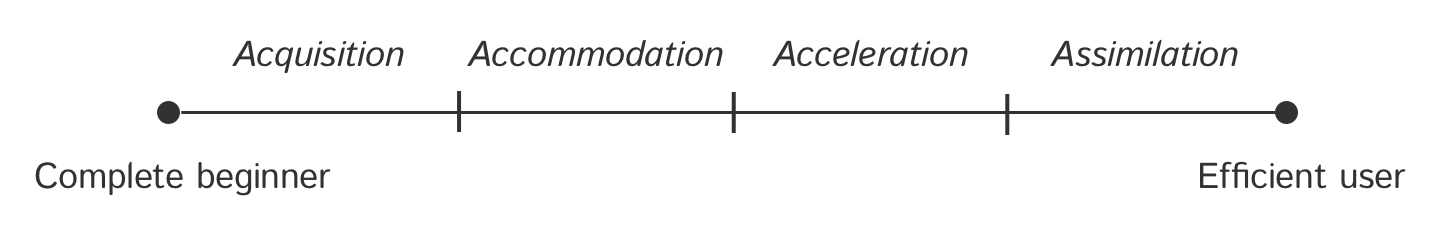
\includegraphics[width=0.8\textwidth]{presentation/Timeline}
  \caption{Onboarding process.}
  \label{fig:process}
\end{figure}

\section{Acquisition}
There is a lot of different factors that determine the willingness for an individual to use and adopt an app. For this section we will discuss the steps of the \textit{adoption process}, and what the app designer can do to impact it.

\subsection{Adoption process}

The adoption process of a user follows five steps; \begin{enumerate*}[label=(\(\arabic*\))]
  \item knowledge,
  \item persuasion,
  \item decision,
  \item implementation and
  \item confirmation,
\end{enumerate*} all of which are explained further in the following subsections below.

\subsubsection{Knowledge}

Knowledge is when an individual first gathers knowledge about the mobile app. They may hear about the app from a friend, or through an advert or by actively looking for a product that satisfies one of the needs of the user. Research by Google and Ipsos has found that apps are often discovered outside the app store; 52\% hear about apps through their family, friends and colleagues, 40\% browse the app store, 27\% use some sort of search engine, 24\% from a company website and 22\% through TV \cite{Tiongson2015}.

After learning about the existence of the app the person may ask questions such as "What is the app?", "How does the app work?" and "Why does it work?". While answering these questions they may acquire \textit{how-to knowledge} and \textit{persuasion knowledge}. How-to knowledge is knowledge about how to use the app and may be acquired through word-of-mouth, reading about the application online or reading its description on the application store of the corresponding mobile platform. Persuasion knowledge is about understanding \textit{how the app works}. This type of knowledge may be harder to acquire, but it is usually not required by the user to use the app.

\begin{displayquote}
  \textbf{DO:} Identify possible touchpoints where the user can find information about the app and communicate the value of the app.
\end{displayquote}

\subsubsection{Persuasion}

Persuasion is when the person form a favorable or unfavorable attitude toward the usage of the mobile app. When this happens, the person is thinking about how they can apply the app to their current situation, and if it meets their needs. At this stage, the person may ask questions such as "What are the app's consequences?" and "What will its advantages and disadvantages be when I apply it to my situation?". Here, peer opinion is important to person. If a friend or relative has had positive experiences with the mobile app they are more likely to form a favorable opinion about it.

Forming a behavioral intention to use the mobile app is based on two major beliefs; \textit{perceived ease of use} and \textit{perceived usefulness}. Perceived ease of use is how much the person believes that using the mobile app will be free of effort and easy to use. Perceived usefulness is how much a person believes that using the app will improve their life. These two beliefs affect each other; when an app is easy to use it can be more useful.

What are some determinants of perceived ease of use and perceived usefulness? Some of them are explained below:
\begin{description}
  \item[Control] - Control is to what extent an individual believe that they have the required knowledge, resources, and opportunities to perform a specific behavior \cite{Venkatesh2000}.
  \item[Intrinsic motivation] - the motivation that comes from the pleasure and satisfaction from performing a behavior (see Section \ref{subsec:motivation} for a more thorough explanation)
  \item[Emotion] - The emotional aspect of technology usage can severly impact the user's attitude \cite{Venkatesh2000}.
\end{description}

It is also worth to point out that perceived ease of use and perceived usefulness are not only determined by the mobile app itself, but also by the persons prior experience with either similar apps and their general experience with using mobile apps. If they have had negative experiences before with a similar app they are more likely to form an unfavorable opinion about the apps perceived ease of use and perceived usefulness, affecting the behavioral intention to use the app.

\begin{displayquote}
  \textbf{Do:} Consider who will be using the app and tailor the experience to that target group.
\end{displayquote}

\subsubsection{Decision}
The decision process leads the person to the decision whether or not to become a user of the app. This decision is usually made after the person has tried the app. This is a crucial part of the adoption process, and its important to eliminate any uncertainty about the app as they use it for the first time. At this stage, it is important to get the user actually using the app as quick as possible. If the app cost money to use, or if the value is hidden behind a cumbersome sign-up process, it must be adopted or rejected in its entirety and is harder to adopt.

\begin{displayquote}
  \textbf{DO:} Reduce the amount of steps required for the user to experience the value of the app.
\end{displayquote}

\subsubsection{Implementation}
Even though a person has decided to download and use an app, actually putting it to use is a whole other thing. For a target behavior to occur (in our case for the person to use the app regularly) the person needs the \textit{motivation} and \textit{ability} to do so. Motivation can be categorized into \textit{intrinsic} and \textit{extrinsic} motivation. Intrinsically motivated people are motivated to do something due to the task being interesting or fun, like playing a video game, while extrinsically motivated people are motivated to do something to achieve a specific external goal, like taking a shower. Extrinsic motivation can be powerful, but when the external reward is removed so does the motivation. It has been found that intrinsically motivated people perform have a higher willingness to spend more time on a task. These categories of motivation are not mutually exclusive; a person may be both intrinsically and extrinsically motivated.

To improve the users intrinsic motivation, the user interface designer can relate the content and objectives of the application to the needs and interests of the learner \ignore{\cite{Keller1983}}. This can be done by using familiar metaphors and analogies \ignore{\cite{Curtis1984}}. Instructions provided to the user that use a personal style (e.g personal pronouns, names of specific people) rather than formal style may stimulate the user to learn. Also, providing immediate, positive and informative feedback in a context may improve intrinsic motivation, but not necessarily increase or decrease performance \ignore{\cite{(Bates, 1979; Condry, 1977; Deci, 1975, 1971; Keller, 1983)}}. Humor, on the other hand, has been found to not improve motivation since it can distract the user and interfere with comprehension \ignore{\cite{Markiewicz, 1974; Sternthal & Craig, 1973}}.

Increasing the motivation of the user is not always the solution to make them perform a target behavior or use your mobile app. Sometimes increasing the users ability to perform the target behavior (making it easier to perform), or increasing the perceived ease of use, is the solution.

While some amount of motivation and ability is required for the user to perform some task, a trigger is required to remind the user to perform the task. Fogg has identified three categories of triggers that help the user

\begin{description}
  \item[Spark as Trigger] High ability/Low motivation, the \textit{spark} should try and motivate the user to perform the behavior.
  \item[Facilitator as Trigger] Low ability/High motivation, the \textit{facilitator} should try and make the target behavior easier to perform.
  \item[Signal as Trigger]  High ability/High motivation, the \textit{signal} should only remind the person to perform the target behavior.
\end{description}

Here are some examples of implemented triggers in mobile applications.

\begin{figure}
\centering
\captionsetup{format=multiline,font=footnotesize}
\begin{minipage}{.33333\textwidth}
  \centering
  \includegraphics[noincl, width=\linewidth,height=8cm]{triggers/spark.png}%
  \caption{\\Spark as Trigger}
  \label{fig:spark}
\end{minipage}%
\begin{minipage}{.33333\textwidth}
  \centering
  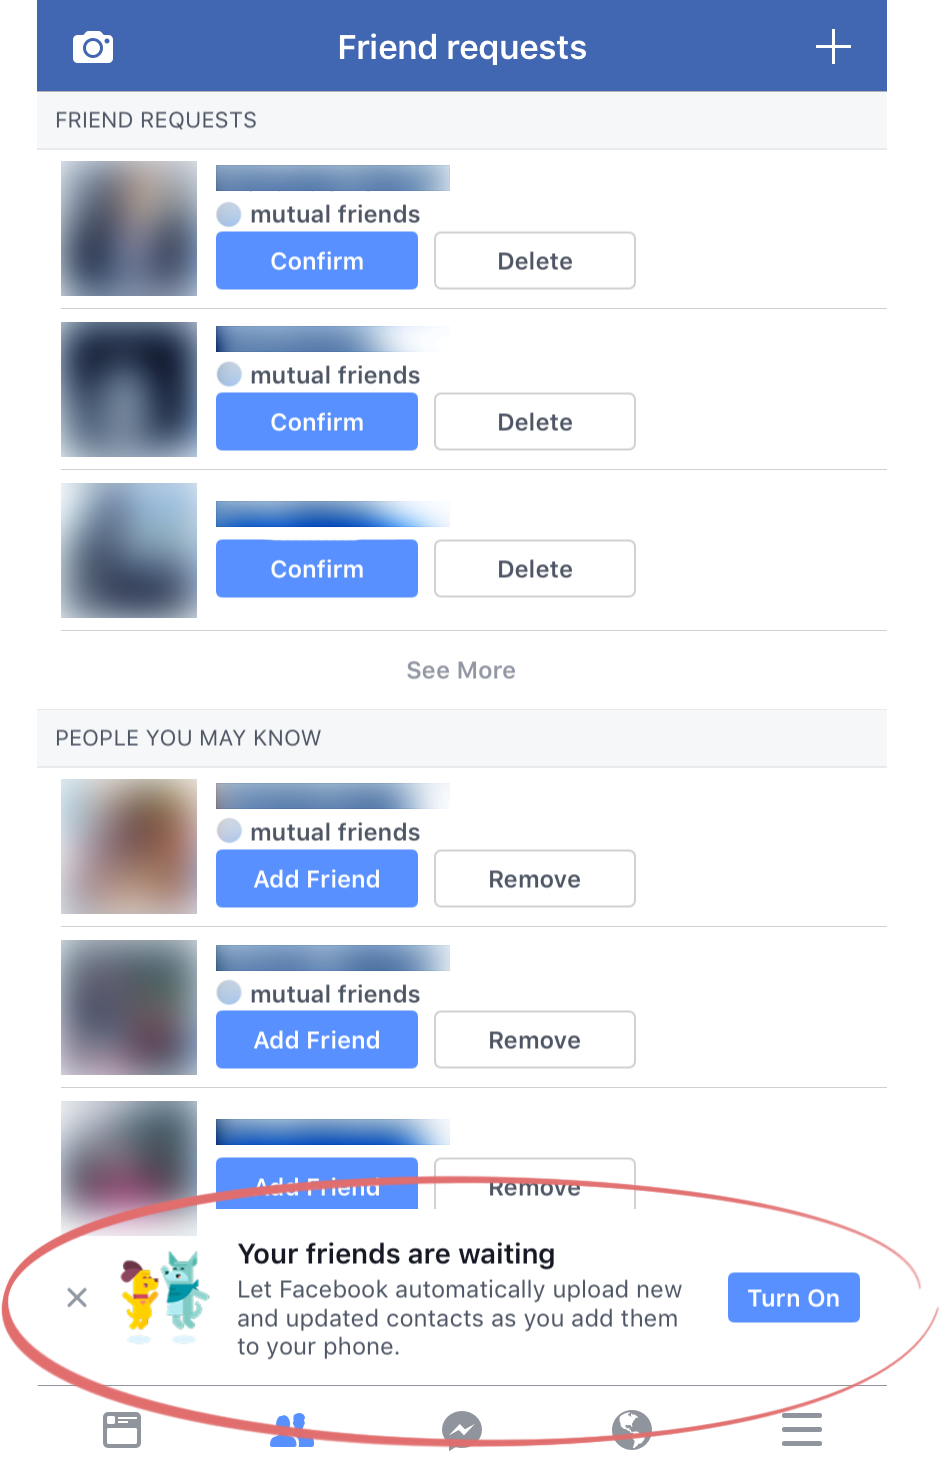
\includegraphics[width=\linewidth]{triggers/facilitator.png}%
  \captionof{figure}{\\Facilitator as trigger}
  \label{fig:facilitator}
\end{minipage}%
\begin{minipage}{.33333\textwidth}
  \centering
  \includegraphics[noincl, width=\linewidth, height=8cm]{triggers/signal.png}%
  \captionof{figure}{\\Signal as trigger}
  \label{fig:signal}
\end{minipage}
\end{figure}

To be able to help the user perform a task we need to think about what influences the difficulty of a task.

\begin{description}
  \item[Time] If the user does not have the time to perform a task, the task will not be easy to perform.
  \item[Money] If the user does not have the money or resources to perform a task it will not be easy to perform.
  \item[Physical Effort] Behaviors that require physical effort may not be easy to perform. If the physical effort is small, the easier it is for the people to perform the behavior. It is important at this stage to consider the different physical disabilities of your target market.
  \item[Brain cycles] A task that is demanding the user to think hard about it might lead the person to think that it is difficult to perform. In some cases, the task at hand might not itself be hard to think about, but the persons mind might be consumed with other issues at the same time.
  \item[Social deviance] If the task required the person to go against the norm, breaking the rules of society, the behavior is not simple to perform.
  \item[Non-routine] People tend to think that activities they perform on a routine to be easy, like brushing your teeth, while new activities might be hard to perform. While seeking simplicity, the person might resort to performing a task that they are more familiar with instead.
\end{description}

These aspects might influence us differently. For example, a person that is in a rush to catch the bus will believe that performing any other task will be difficult. Or a person might find it difficult to input voice commands while in the presence of strangers. The one aspect that we have the most limited resources of when a behavior is triggered will determine how difficult the task is.

Even though with the mobility of smartphones, its wide range of possible uses and the big opportunity of using contextual triggers we must be cautious of the triggers we use. Sparks may annoy us because they will try and motivate for a behavior that we do not want to perform. Users will be most tolerant of triggers when they act as signals or facilitators.

\begin{displayquote}
  \textbf{DO:} Identify where your user will most likely be using your app and what resources they might be lacking at that particular time. If you are designing an app for looking up transit times for buses, consider that they might be in a rush to the bus stop while using the app.
\end{displayquote}

\begin{displayquote}
  \textbf{DO:} Identify where the user experience can be enhanced with the correct triggers.
\end{displayquote}

\subsubsection{Confirmation}

The final stage of adoption is the \textit{confirmation} stage. At this stage, the individual will seek confirmation that their choice to use an app is correct, but if the individual find conflicting messages about the app they will experience \textit{dissonance}. The feeling of dissonance is unpleasant to the user, and will try to avoid by either changing their beliefs, attitude or knowledge. The person may avoid dissonance by only seeking information that support their decision to adopt or avoid information that is not consistent with the person's beliefs. Avoiding conflicting messages can still reach the individual, even if they avoid it, and they may doubt their decision to use the app. Examples of conflicting messages might be opinions from a friend or bad ratings of the app.

The decision to continue using an app is highly dependent on the user's \textit{satisfaction} with the app. Satisfaction is the users expected experience vs. their actual experience, and the app has to exceed the expectations of the user to feel satisfied and confirm their decision to use the app.

% \subsection{User research}
% To successfully satisfy the need of your user with your app you need to identify the need they are trying to satisfy. This implicitly means that you have to identify you user-base and in what context they will be using your mobile app. In the product development cycle, this is usually done through \textit{user research}.
%
% User research focuses on understanding user behaviors, needs and motivations through different observation techniques\ignore{\footnote{\url{https://www.usability.gov/what-and-why/user-research.html}}}. While there are plenty of different methods for learning about your users, we will endorse creating \textit{personas} to represent your target market.

\section{Accommodation}
Accommodation is giving the user what they need to succeed with the app. To be able to do this we need to be able to understand how users behave, interact and learn. We also discuss how users decide whether or not they will continue using the app.

\subsection{Performance}

When the user uses the app, they will try to achieve a goal. The goal might be intrinsically motivated (play a mobile game for fun) or extrinsically motivated (use a banking app to pay the bills). What ever the goal might be, the user try to achieve their goal following this conceptual seven step cyclic model:

\begin{minipage}{\linewidth}
\centering
\captionof{table}{Action model} \label{tab:title2}
  \begin{tabular}{ p{0.8\linewidth} } \toprule
    \ \ \ \emph{\textbf{Goal}}\\
    1. Forming the goal \\
    \ \ \ \emph{\textbf{Action}} \\
    2. Forming the intention \\
    3. Specifying the action \\
    4. Executing the action \\
    \ \ \ \emph{\textbf{Evaluation}} \\
    5. Perceiving the system state \\
    6. Interpreting the system state \\
    7. Evaluating the outcome \\
    \bottomrule
  \hline
  \label{table:questions}
  \end{tabular}
\end{minipage}

The steps cyclic model can be categorized into \textit{Goal}, \textit{Action} and \textit{Evaluation}, and each category will be explained further in the following subsections:

\subsubsection{Goal}

The goal is the start of the journey for the user. A goal that has been \textit{incorrectly} formed may make it harder for the user to reach that goal. Predicting or helping the user with goal transformations is a problem that has yet to be solved \cite{Polson1990}.

\subsubsection{Action}

When the user tries to achieve the goal, they will try to figure out what actions they need to perform the achieve that goal. When helping the user performing the correct action, we have to consider two things:

\begin{enumerate}
  \item Will the amount of possible options at any given time overwhelm the user?
  \item Do all possible interactive elements have the proper \textit{affordance}?
\end{enumerate}

If the user has a large number of possible actions to take at any given time, they will have a hard time figuring out which action will lead the user closer to the goal. Even though the thought of a lot of functionality in an app, providing excessive functionality is a danger as the clutter and the resulting complexity make the learning and usage more difficult for the user.

\begin{displayquote}
  \textbf{DO:} Only present the user with relevant functionality and information, do not overwhelm your users.
\end{displayquote}

Affordance is the communication a design element provide to the user about \textit{how} to interact with the element and \textit{what} will happen when they interact with the element. When designing an element of your interface, ask the following questions:

\begin{enumerate}
  \item Is the functionality that the element provides relevant to the user? (If not, consider if the element should really be a part of the interface)
  \item Does the element advertise its purpose, so that the user understand when to interact with it? (e.g. if you're designing button, will the user understand when to press said button?)
  \item Will the user understand from the design of the element what will happen when they interact with it? (e.g. making the color of a button that deletes something red)
  \item Will the location and size of the element allow the user to interact with it?
  \item Will the user understand how to interact with the element? (e.g. making a button raised to indicate that it can be pressed)
\end{enumerate}

\begin{displayquote}
  \textbf{DO:} "Make available actions easy to discriminate" \cite{Polson1990}. The user should be able to determine which action will take the user closer to their goal.
\end{displayquote}

\subsubsection{Evaluation}

When the user has performed an action, they will evaluate whether or not they have gotten closer to their goal. To help the user evaluate the state, it should be clear what their actions resulted in (e.g. if they navigated somewhere, they should be able to tell where they have navigated).

\begin{displayquote}
  \textbf{DO:} Show the user the result of their action in a clear way.
\end{displayquote}

If a user error occurs, that is; if they have taken a misstep toward their goal, the user should be able to recover from that error.

\begin{displayquote}
  \textbf{DO:} Help the user recover from user errors.
\end{displayquote}

\begin{figure}[h]
  \centering
    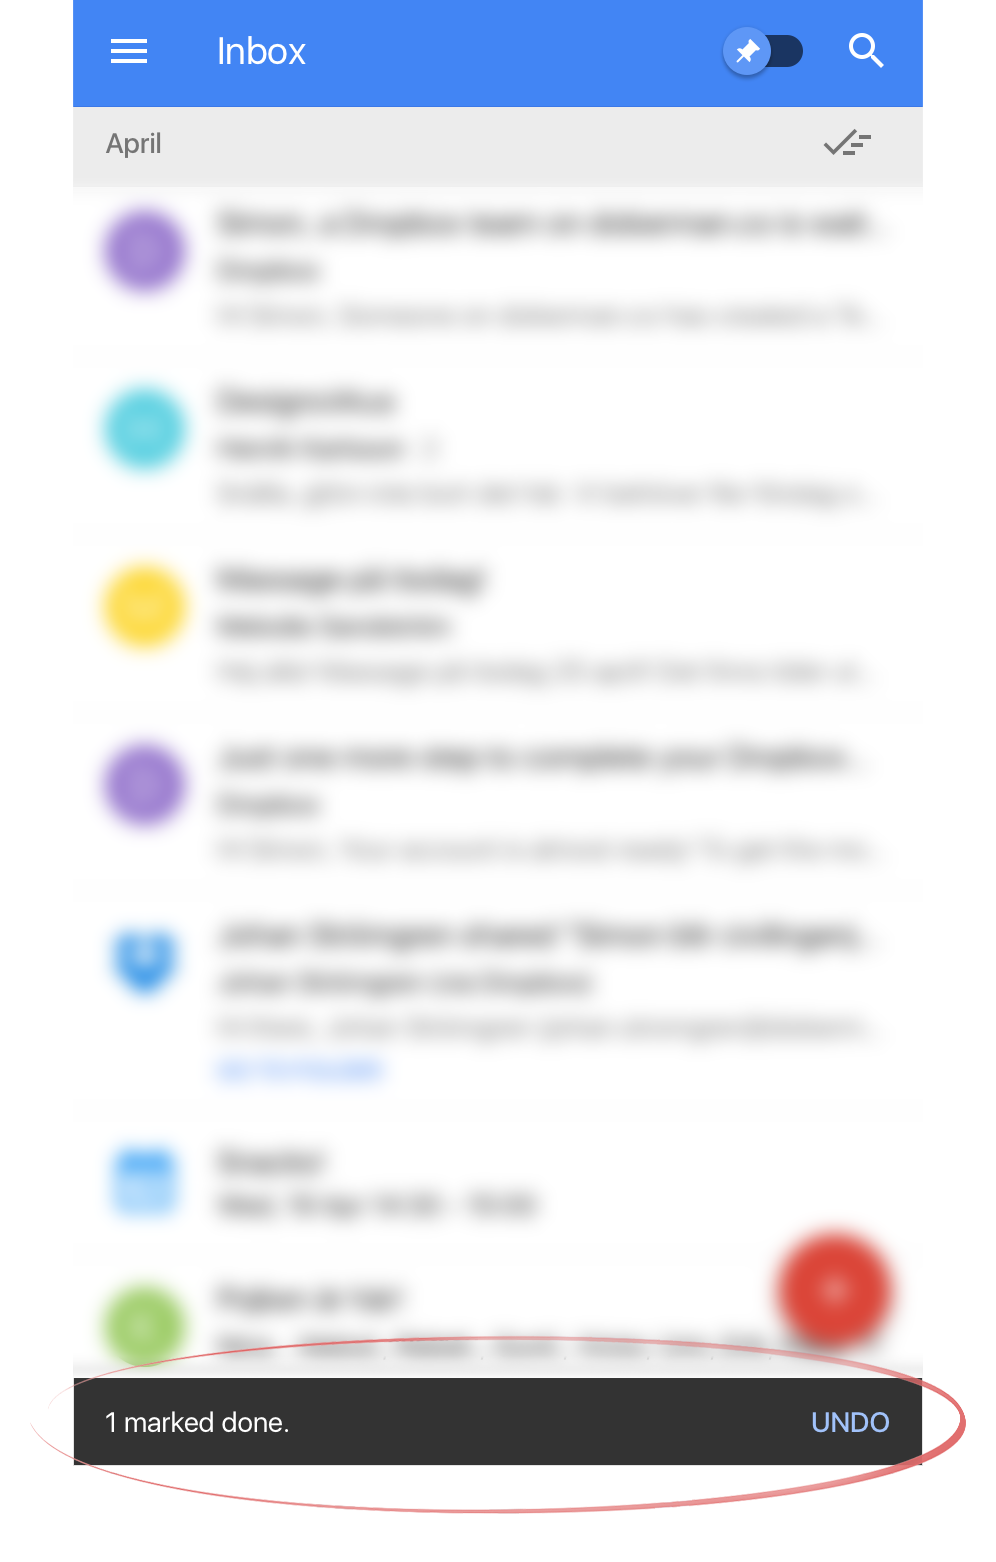
\includegraphics[width=0.3\textwidth]{examples/action-confirmation}
  \caption{An example from the Google Inbox app, where a dialogue tells the user what has happened when they have marked an email as done, with the possibility to undo the action.}
  \label{fig:examples/action-confirmation}
\end{figure}

See \ref{fig:examples/action-confirmation} for an example from the Google Inbox app which showcases a confirmation of what the user's action did, and a possibility to recover if this was a user error.

\subsection{Learnability}
Learnability, in the domain of interaction design, is to have the user learn how to perform the actions of the interface. As the user learn more about the interface and the information system, they will be able to reduce the amount of user errors, reduce task completion time and number of tasks completed successfully \cite{Leung2010}.

% \subsection{Behavior}
%
% There are three levels of performance levels that can be performed by the users.
%
% \begin{description}
%   \item[Skill-based behavior] Description
%   \item[Rule-based behavior] Description
%   \item[Knowledge-based behavior] Description
% \end{description}
%
% Knowledge-based behavior is where most user errors may occur

\ignore{

Rasmussen \cite{Rasmussen1983} has identified three typical levels of performance. \textit{The skill-based behavior} represent the subconscious actions and activities which we perform on a "smooth, automated, and highly integrated patterns of behavior". This level of performance is based on a simple feedback loop, where a stimuli facilitate a motor output. \ignore{Provide example of this}

\textit{Rule-based behavior} are patterns of behavior which emerge from previous and similar actions performed in a previous similar occasion. The user acts in a goal-oriented way where the user tries to achieve a goal, which is usually not explicitly stated, with the rules that has empirically evolved through previous successful experiences.

The main differences of skill-based and rule-based behavior are that the person may not consciously be aware of the actions the user perform when performing actions on a skill-based level, and may not be able to recollect why such an action has been taken. The higher level rule-based actions are generally based on "explicit know-how, and the rules used can be reported by the person".

The third, and final level of performance as Rasmussen \cite{Rasmussen1983} has identified, is \textit{knowledge-based}. Knowledge-based performance is used during situations that the user is not familiar with, and where any know-how or rules cannot be used from previous experiences. Rasmussen \cite{Rasmussen1983} states that "In this situation, the goal is explicitly formulated, based on an analysis of the environment and the overall aims of the person. Then a useful plan is developed by selection such that different plans are considered, and their effect tested against the goal, physically by trial and error, or conceptually by the means of understanding the functional properties of the environment and prediction of the effects of the plan is considered." At this level of abstraction, the user represent the system in an internal construct called \textit{mental model}.

These three levels of performance are similar to the types of user-product interactions identified by Forlizzi \cite{Forlizzi2004}; \textit{Fluent}, \textit{Cognitive} and \textit{Expressive} interaction.

}

\section{Assimilation}
Assimilation is the process of helping the user feel welcome in their new community and environment. If the app in question does not provide a community, some aspects of this section may not apply the app.

\subsection{Co-experience}

\textit{Co-experience} are created together by individuals who share an experience. The individuals may be friends or strangers who share a common interest, and can interact with each other through editing, sharing and viewing content.

\begin{displayquote}
  \textbf{DO:} Help the user find individuals that they can share co-experiences with. This can be done through allowing them search for their interests or finding their friends on the platform.
\end{displayquote}

\subsection{Community}

The community that the app provides can greatly affect the adoptance for the user. The community must meet the needs that the individual seeks, and the subsequent needs can be categorized as follows:

\begin{description}
  \item[Purposive value] is the drive for the individual to gain or share information.
  \item[Self discovery] concerns the individual purpose to learn things about him/herself.
  \item[Maintaining interpersonal connectivity] is the drive to stay in touch with friends or performing activities with other individuals.
  \item[Social enhancement] is the individuals drive to impress members within the community and feel important in the community.
  \item[Entertainment] refers to the individuals drive to relax, have fun, playing with others in the community.
\end{description}

One clear design recommendation, gives to us by Lampe et al, is to support as many of these multiple anticipated needs as possible, and not assume that the users will align to one or the other if their need is not supported \cite{Lampe2010}.

\begin{displayquote}
  \textbf{DO:} Identify the needs your users are looking for in the community your app provides.
\end{displayquote}

\section{Acceleration}
Acceleratin is the act of helping your users perform tasks better and faster and get more value of the app.

\subsection{Personalization}
Smart-phones are devices that are in our pockets at all times, and are inherently personal. Features of a mobile app that can be classified as "personalization" can be everything from simply be displaying the name of the user in a menu to complex recommendations systems.

To be able to provide the user with personal value, information needs to be gathered of the user. This may be quite hard, since users value their personal data very highly. The value that the user is getting in exchange for personal information and value should be communicated and clear to the user so that they are more likely to provide personal information. A strategic way to go about this, as developed by Karat et al \cite{Karat2003}, is to ask the user of a small amount of personal data and reward the user with value accessible through the app. This might lead to a feedback loop where the more personal information is given the more value the user get.

\begin{figure}[h]
  \centering
    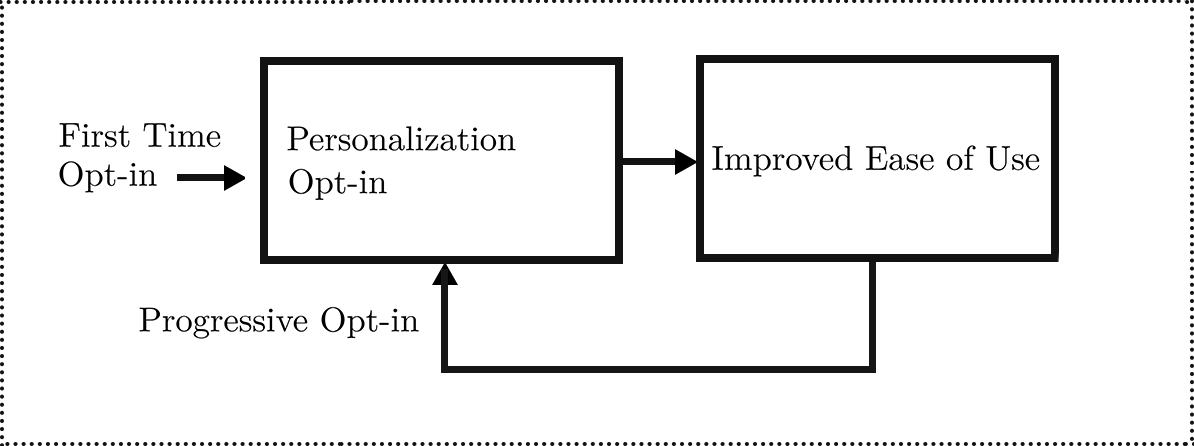
\includegraphics[width=0.6\textwidth]{personalization-value}
  \caption{Personalization Value Model (modified from \cite{Karat2003}).}
  \label{fig:personalization-value}
\end{figure}

% \subsection{Skill mastery}
%

\section{Onboarding techniques}

This is an overview of common onboarding techniques employed by apps. In the following subsections, we will discuss these techniques and when their use is appropriate.

\subsection{Coach marks}
When the user use the app for the first time, they are presented with an overlay with a description of the most important features of the app, called \textit{coach marks}. The marks coach the user on how to access the an app functionality and how they work.

Coach marks should be avoided if possible since the overabundance of information presented might overwhelm the user. Interactive elements and their function should, in the best case scenario, be communicated through their design and affordances.

\subsection{Interactive tutorial}

Interactive tutorials are a tool to help the user experience the app incrementally and in a controlled environment.

Interactive tutorials are especially suited for mobile games, where the interactive elements are presented to the user in a controlled environment. It is also suitable for mobile apps where a core interaction is unconventional and need

\begin{figure}[ht]
\begin{subfigure}{.25\textwidth}
  \centering
  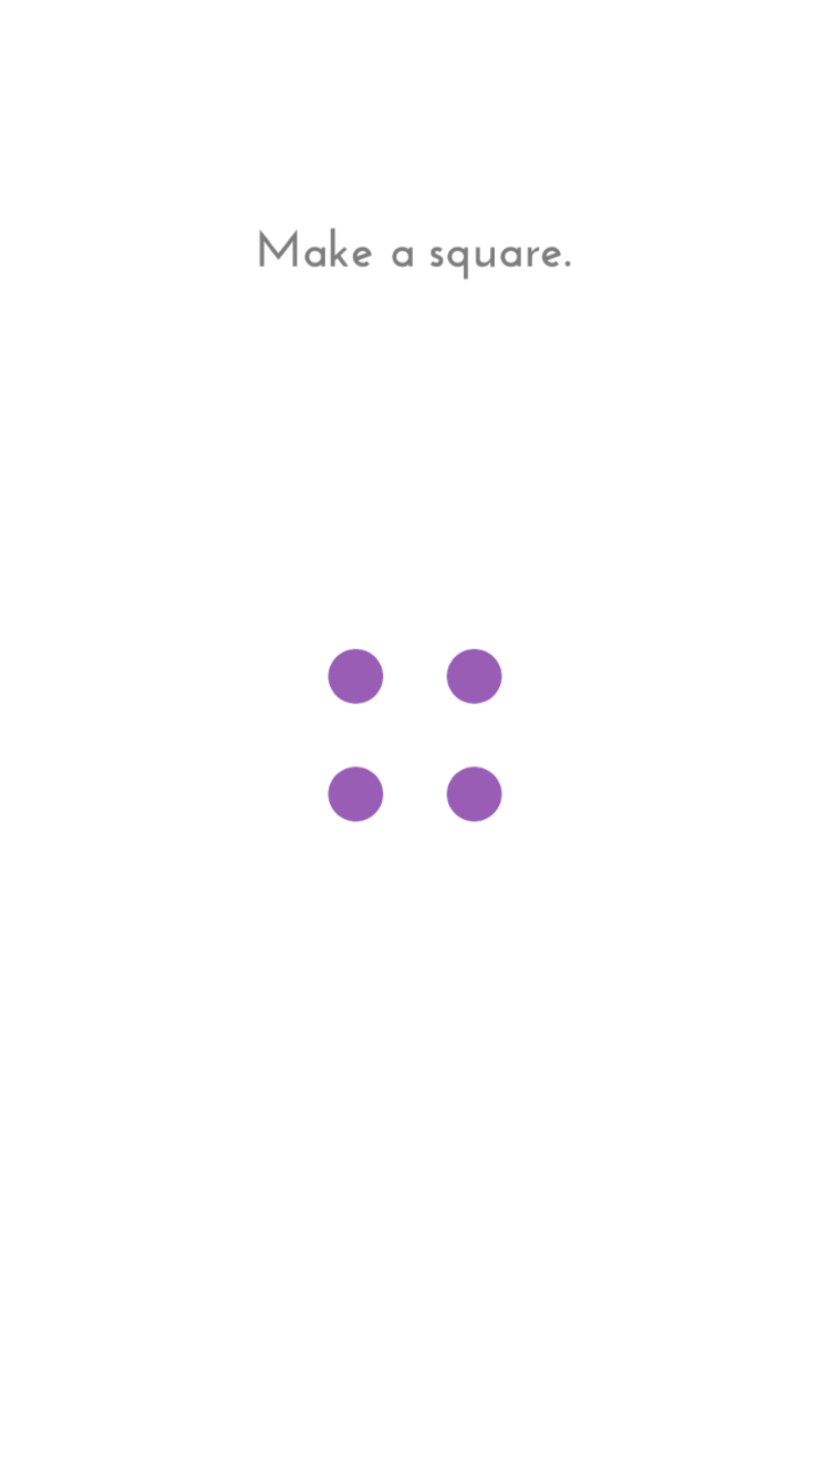
\includegraphics[width=0.95\linewidth]{best-practice/interactive-tutorial/dots-1}
  \label{subfig:best-practice/interactive-tutorial/dots-1}
\end{subfigure}%
\begin{subfigure}{.25\textwidth}
  \centering
  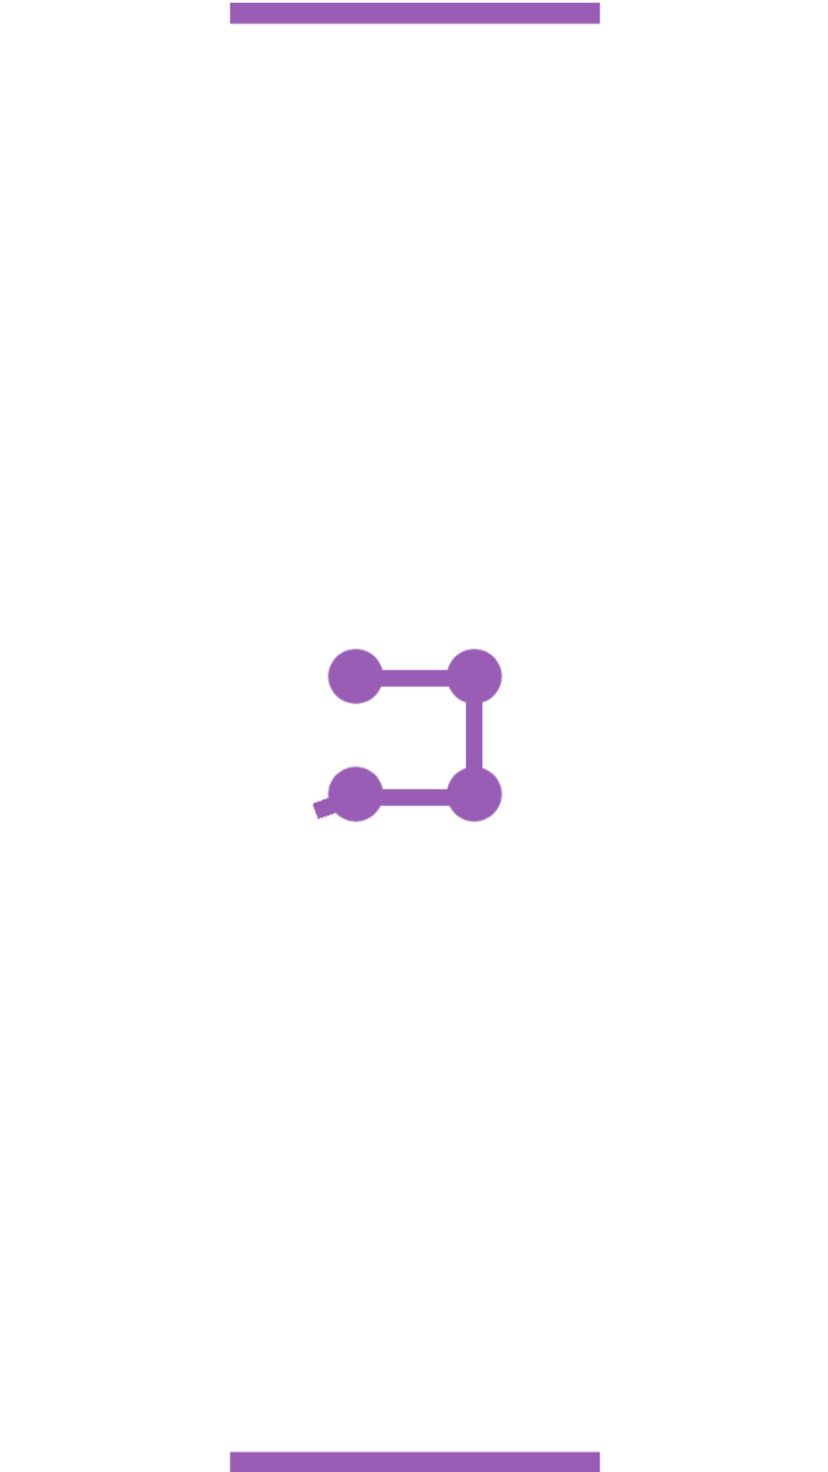
\includegraphics[width=0.95\linewidth]{best-practice/interactive-tutorial/dots-2}
  \label{subfig:best-practice/interactive-tutorial/dots-2}
\end{subfigure}%
\begin{subfigure}{.25\textwidth}
  \centering
  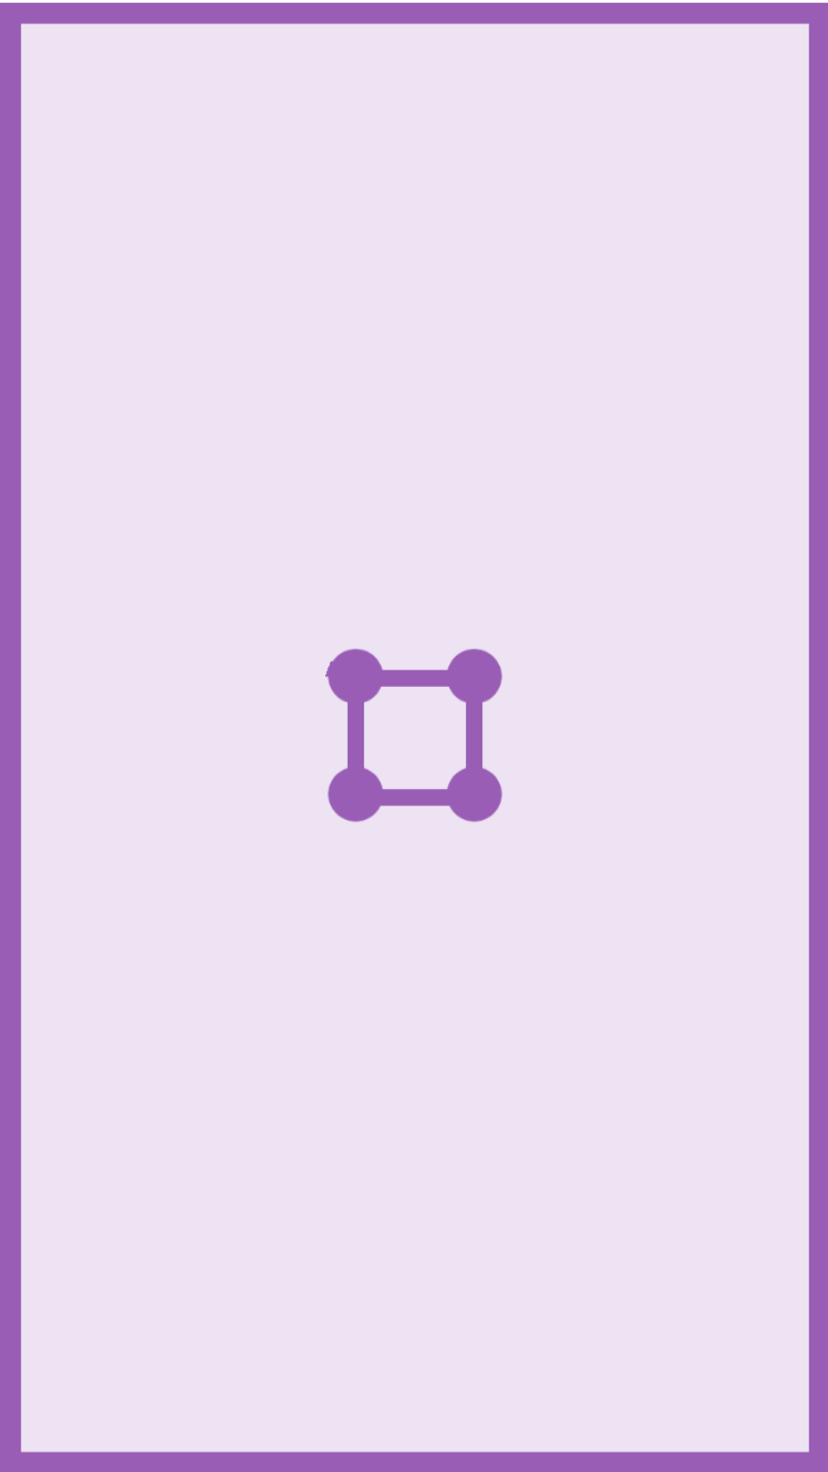
\includegraphics[width=0.95\linewidth]{best-practice/interactive-tutorial/dots-3}
  \label{subfig:best-practice/interactive-tutorial/dots-3}
\end{subfigure}%
\begin{subfigure}{.25\textwidth}
  \centering
  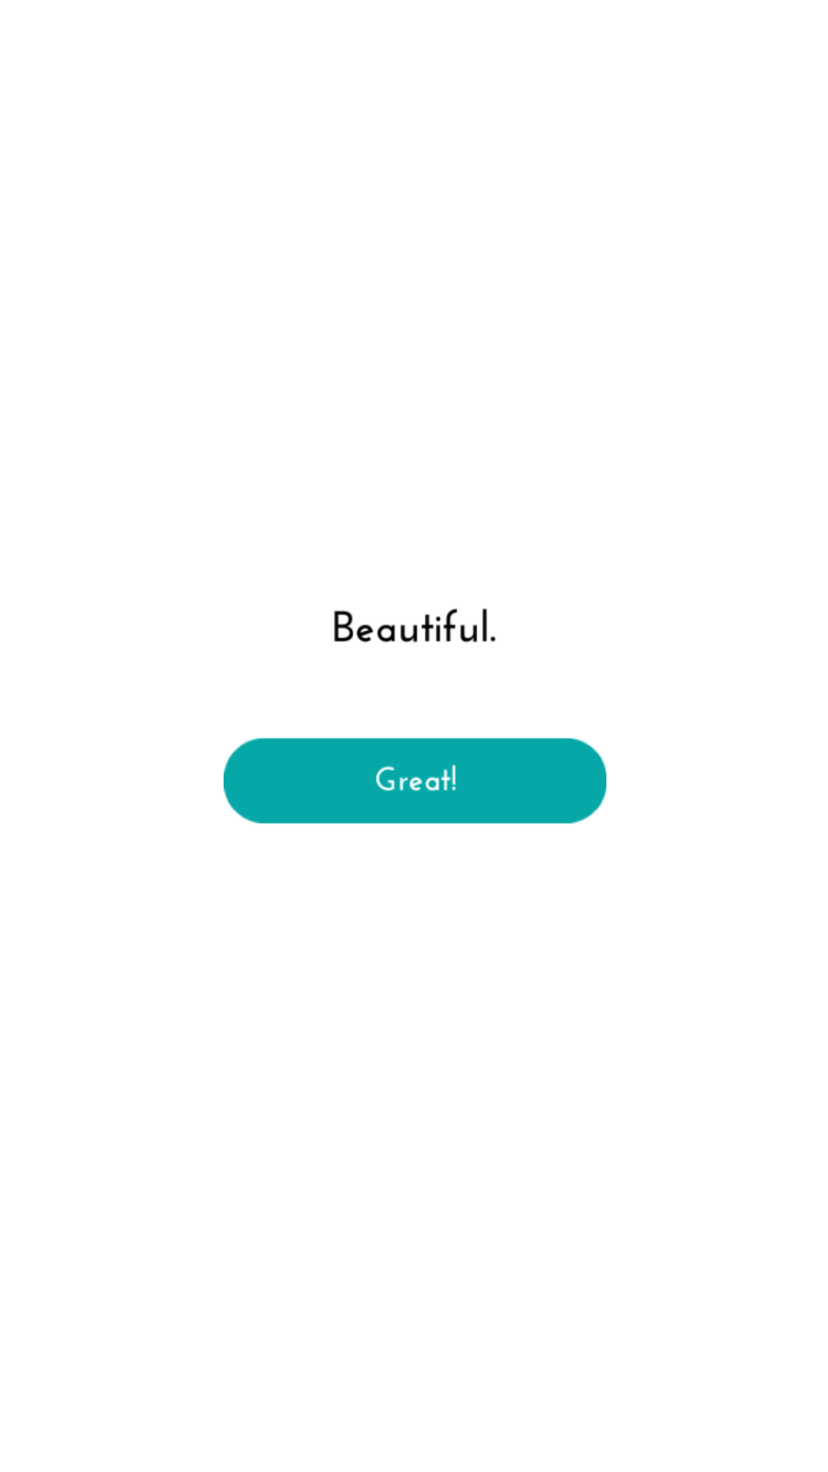
\includegraphics[width=0.95\linewidth]{best-practice/interactive-tutorial/dots-4}
  \label{subfig:best-practice/interactive-tutorial/dots-4}
\end{subfigure}%
\caption{A part of the interactive tutorial in the mobile game "Dots"}
\label{fig:general-overview}
\end{figure}

\subsection{Contextual instructions}

Contextual instructions are similar to coach marks as they also point out important functionality and how to access them, but they are \textit{contextual} as they point out the functionality when the user is most likely to try and access the functionality.

Contextual instructions are useful when the user is trying to access a certain functionality, and non-intrusive information can be provided to the user that the interface cannot alone provide affordance for.


\subsection{Tutorial cards}

Tutorial cards are used to showcase the core functionality of the mobile app in a number of "cards".

\begin{figure}[ht]
\begin{subfigure}{.25\textwidth}
  \centering
  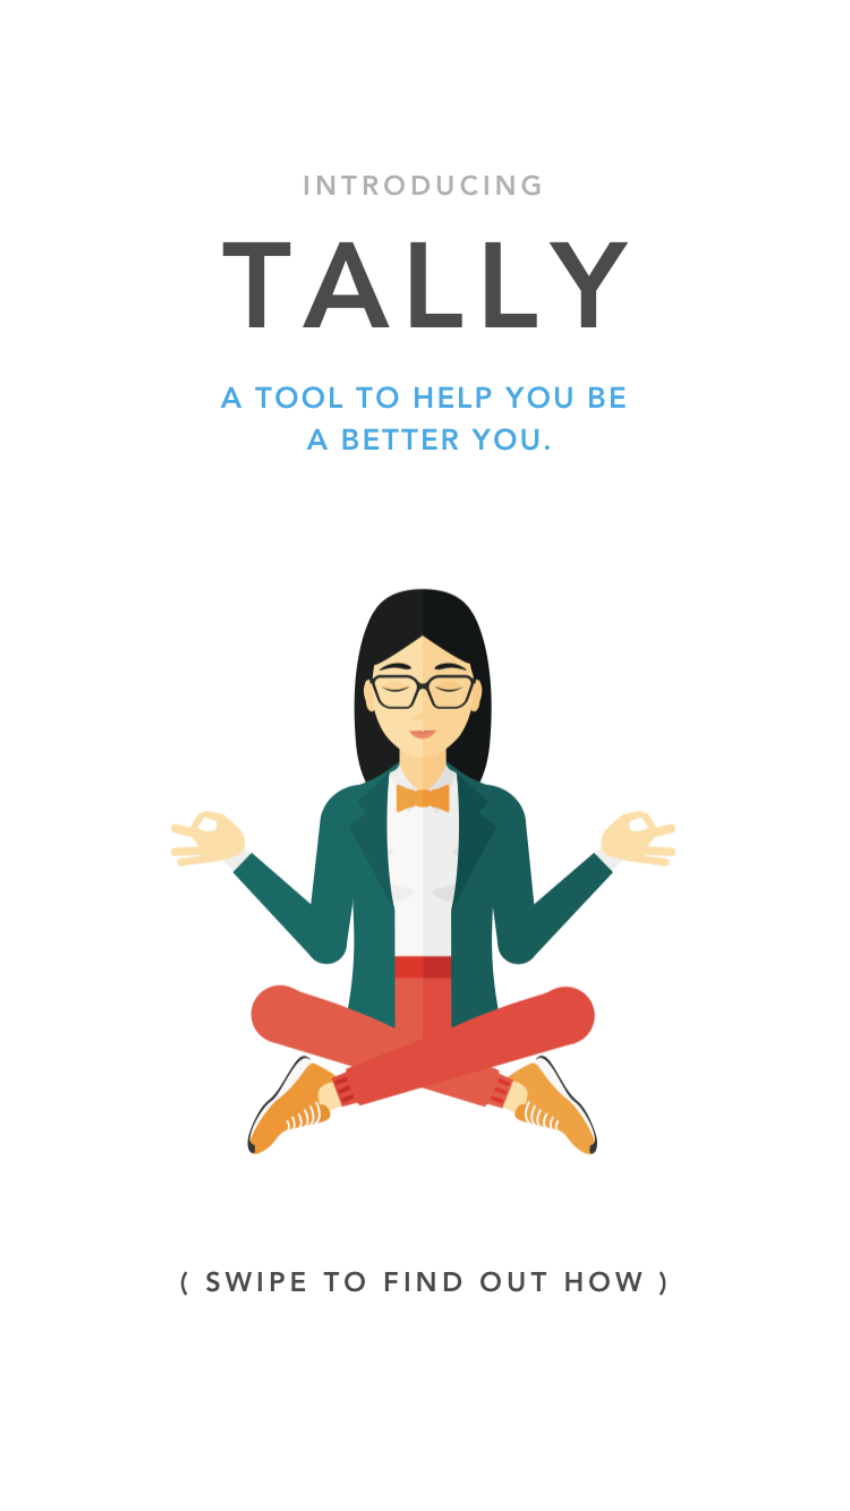
\includegraphics[width=0.95\linewidth]{best-practice/tutorial-cards/tally-1}
  \label{subfig:best-practice/tutorial-cards/tally-1}
\end{subfigure}%
\begin{subfigure}{.25\textwidth}
  \centering
  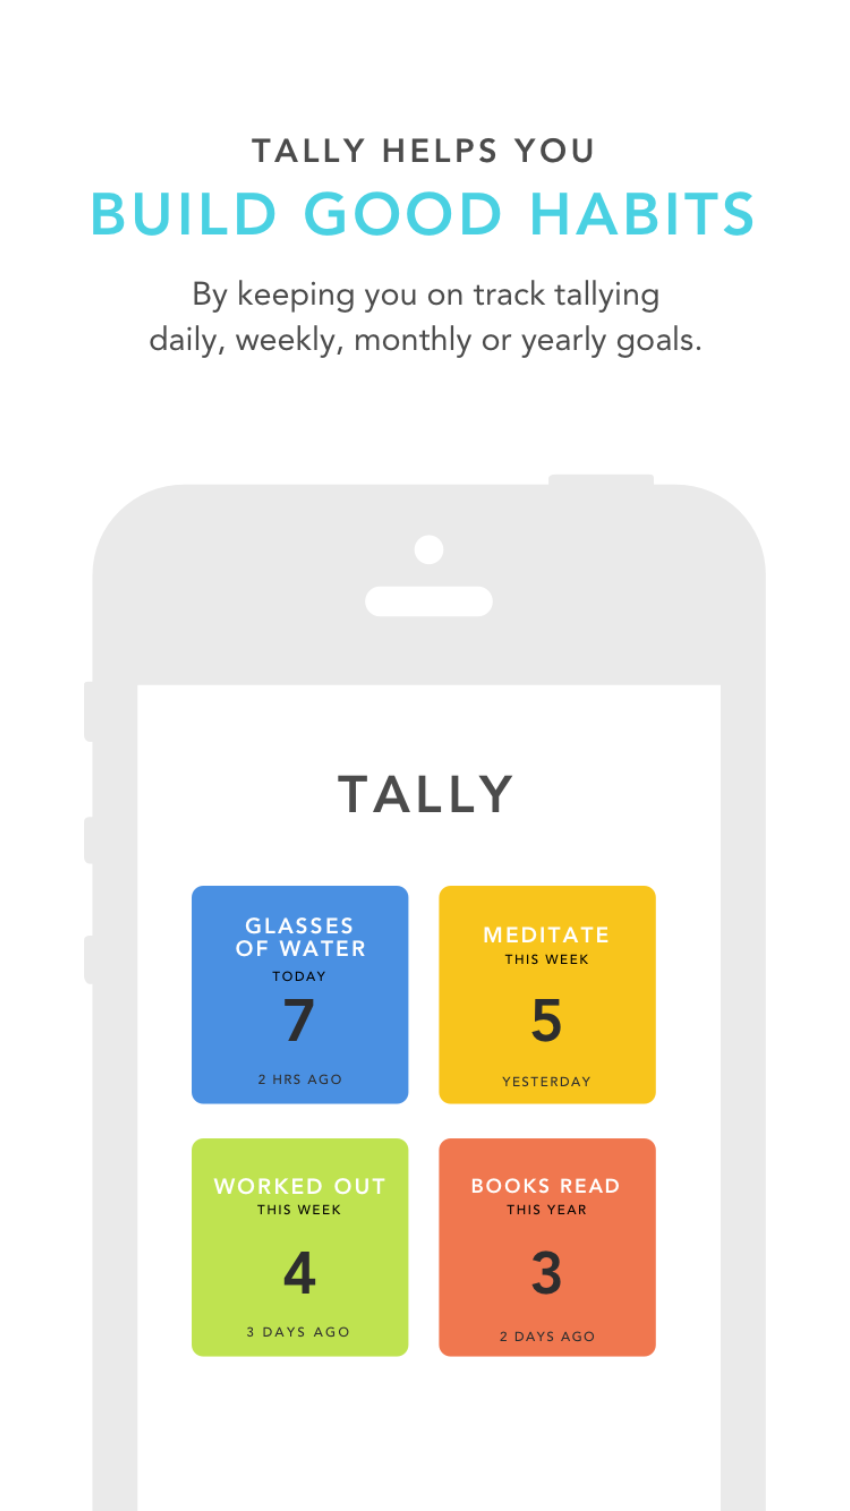
\includegraphics[width=0.95\linewidth]{best-practice/tutorial-cards/tally-2}
  \label{subfig:best-practice/tutorial-cards/tally-2}
\end{subfigure}%
\begin{subfigure}{.25\textwidth}
  \centering
  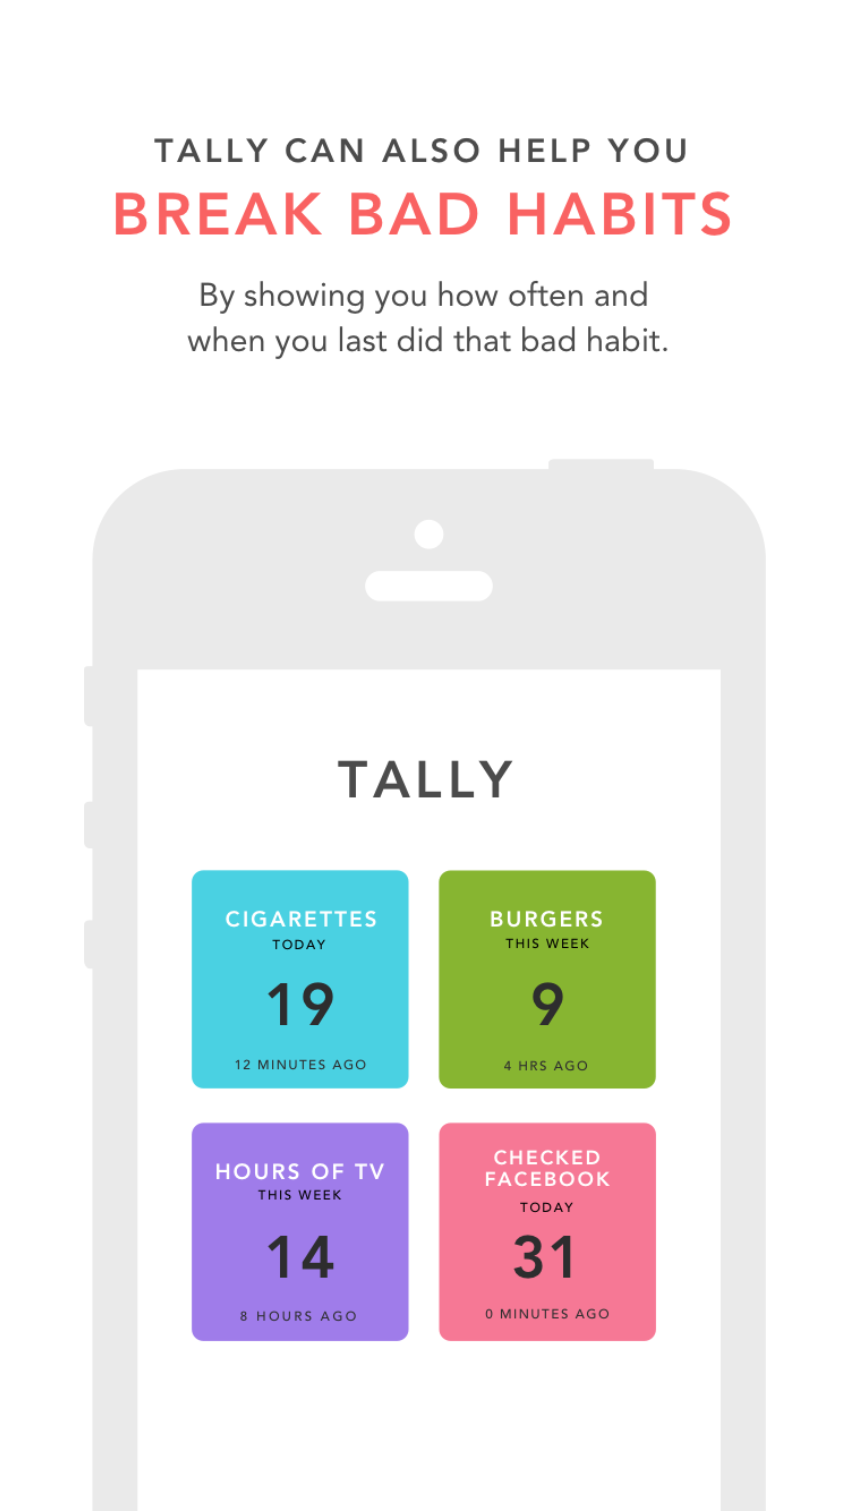
\includegraphics[width=0.95\linewidth]{best-practice/tutorial-cards/tally-3}
  \label{subfig:best-practice/tutorial-cards/tally-3}
\end{subfigure}%
\begin{subfigure}{.25\textwidth}
  \centering
  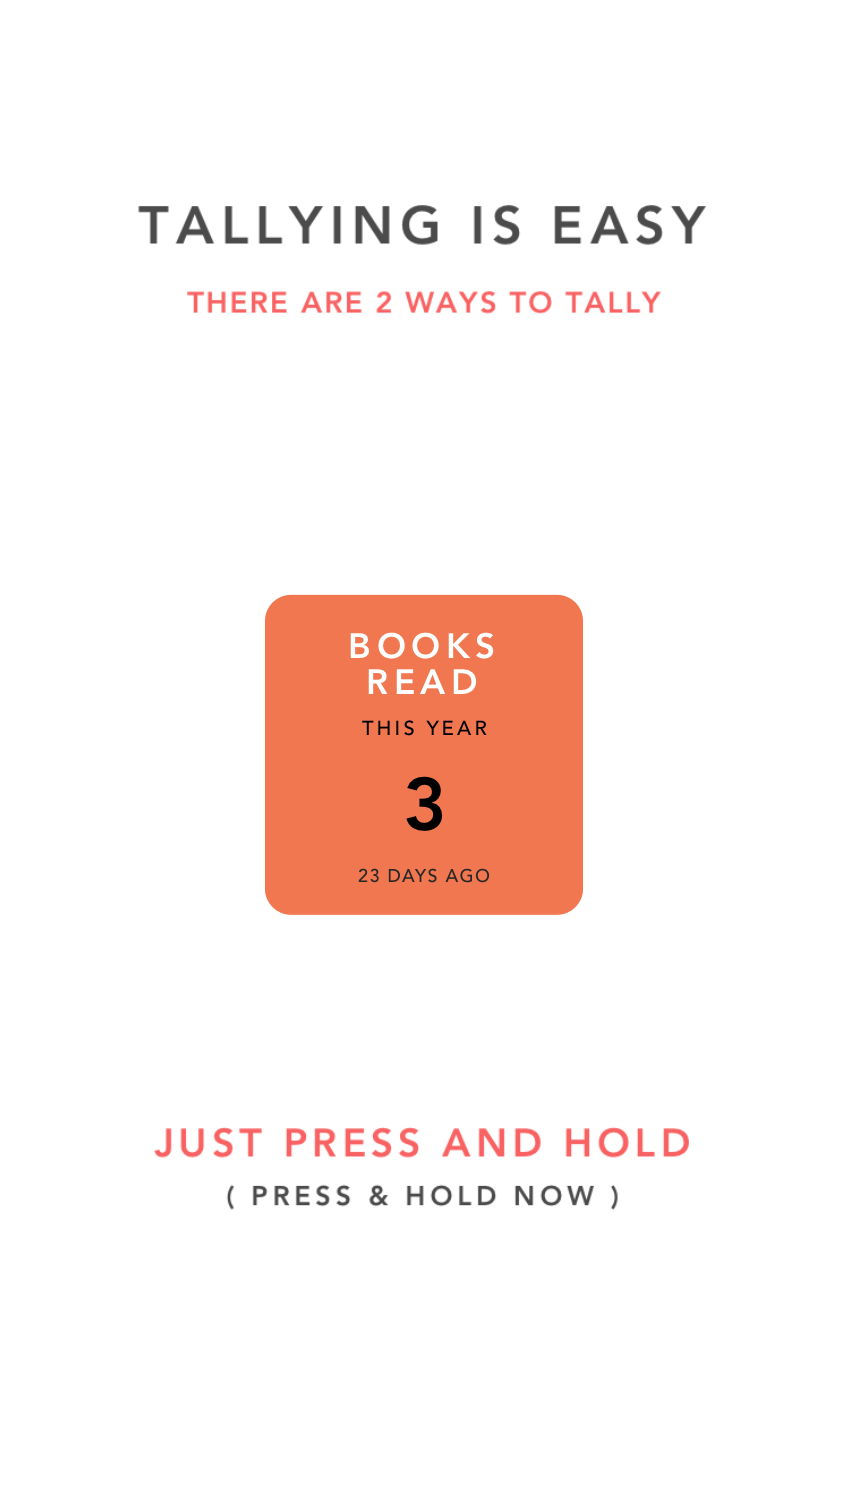
\includegraphics[width=0.95\linewidth]{best-practice/tutorial-cards/tally-4}
  \label{subfig:best-practice/tutorial-cards/tally-4}
\end{subfigure}%
\caption{Tutorial cards in the mobile app "Tally"}
\label{fig:general-overview}
\end{figure}

\subsubsection{Benefits}
Tutorial cards will help the user when they first open the app to understand what is possible with the app, and when the correct understanding of the app's functionality is critical.

\subsubsection{Disadvantages}
The tutorial cards do not consider the context of the user, and if the user just want to get on to the core functionality it is very likely that they will skip the tutorial cards in its entirety, and might miss out on important information. Also, the tutorial cards mostly provide what is possible through the app, not \textit{how} to achieve these possibilities.
